% Chapitre de découverte des services offerts
\chapter{Découvrir les différents services}
%\addcontentsline{toc}{chapter}{Découvrir les différents services}

Le portail est le centre névralgique de l'environnement de la Boîte. 
Au début il est pour ainsi dire vide sauf la présence dans l'espace, en haut, d'une barre avec plusieurs onglets~:
\begin{figure}
	\centering
	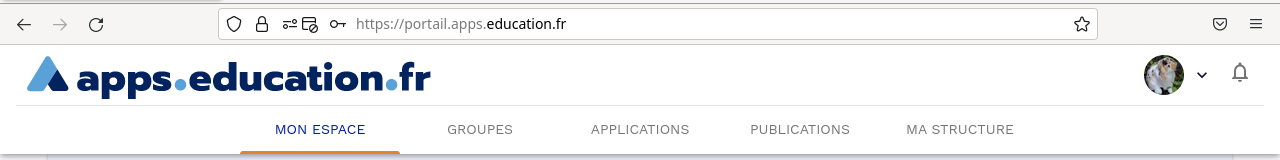
\includegraphics[width=\linewidth]{./Captures/portail.barre.haute.png}
%	\caption{}
\end{figure}
Une fois la première connexion établie, il sera demandé de vérifier et compléter le profil. 
De nombreux champs, ceux utilisés lors de l'enregistrement ne sont pas modifiables, et généralement il reste quelques options à régler en bas~: la structure de rattachement et les options de publication

Deux onglets seront intéressants dans les premiers temps, celui des groupes et celui des applications puisque leur rôle est d'ajouter de nouvelles vignettes au sein de l'accueil (onglet de gauche).

\begin{figure}
	\centering
	
\includegraphics[width=\linewidth]{./Captures/portail.barre.seule.png}
%	\caption{}
\end{figure}

Une fois que vous aurez ajouté les applications ou les groupes, votre portail pourra évoluer et par exemple ressembler à celui-ci~:
\begin{figure}
	\centering
	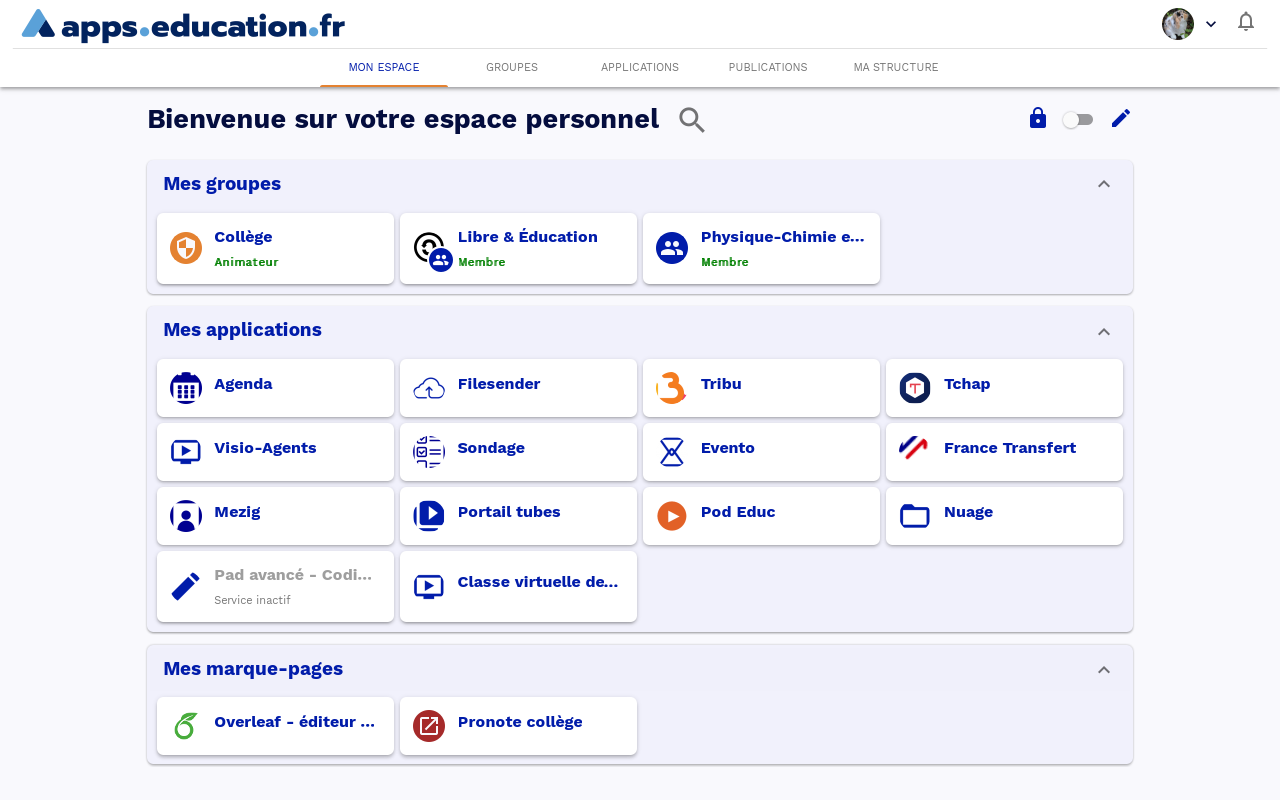
\includegraphics[width=0.7071\linewidth]{./Captures/portail.accueil.png}
%	\caption{}
\end{figure}

\paragraph*{Comment ajouter de nouvelles briques ?}
La méthode est assez simple, il suffit de jeter un \oe{}il soit aux onglets, soit au menu de l'utilisateur à droite.

% portail-ajout-groupe.tex
\section{Ajouter un groupe à son profil}

\subsection{Affichage de tous les groupes disponibles}
Une fois l'onglet \og~\bsc{groupes}~\fg{} sélectionné comme le montre la capture d'écran la liste des groupes disponibles, 193 ici au message \textbf{Explorer les groupes (193)}. 
À sa droite une loupe vous permet de saisir un mot clé du nom du groupe si vous le connaissez et le filtre agira en affichant uniquement les éléments concernés.
\begin{figure}
	\centering
	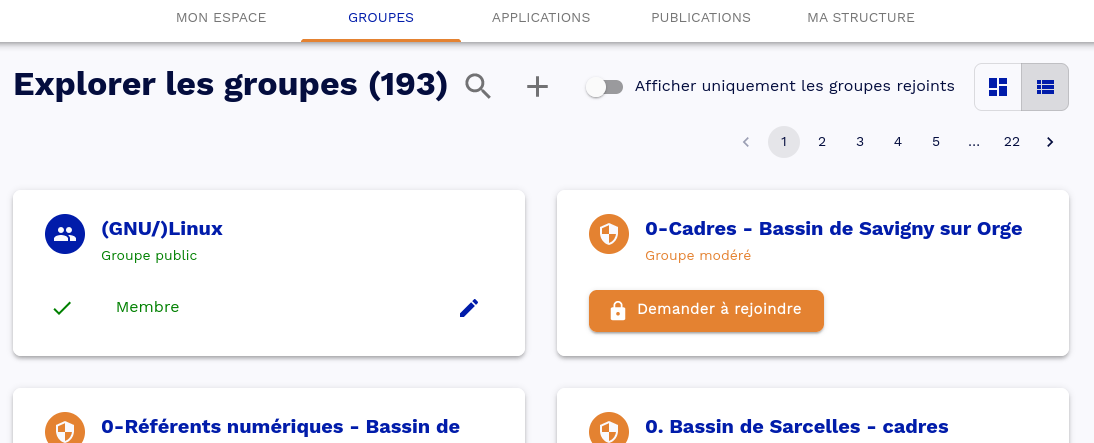
\includegraphics{./Captures/portail.groupes.selection.png}
	\caption{Affichage des différents groupes disponibles}
\end{figure}

À la droite de la loupe, un grand signe plus vous permet de créer un groupe, où, par défaut en tant que créateur, vous serez aussi l'administrateur.

\begin{quote}
	\emph{Là où l’on trouve un grand pouvoir, on trouve une grande responsabilité.}\newline
	\begin{flushright} Winston Churchill (1906) \end{flushright}
\end{quote}


\subsection{S'inscrire à un groupe}
Parmi les groupes se trouvent des groupes publics ouverts à tous, donc les accentuations colorées sont bleu où l'inscription est automatique dès que vous cliquez sur le bouton \fbox{$\boxed{\rightarrow}$ \hspace{0.1cm} Rejoindre le groupe}
\begin{figure}
	\centering
	
\includegraphics[width=0.500\linewidth]{Captures/portail.groupe.exemple.public.png}
	\caption{Exemple de groupe public}
\end{figure}
C'est le cas de ce groupe Test2 ou bien auparavant du groupe \textbf{(GNU)/Linux}, mais se trouvent aussi des groupes modérés à inscription suite à une validation, ces groupes apparaissent avec des icônes oranges circulaires représentant l'équivalent d'un bouclier, et aussi par une coloration orange. 
De même le bouton n'affiche pas \emph{Rejoindre le groupe} comme auparavant mais un cadenas et \textbf{Demander à rejoindre} puisqu'un modérateur ou un administrateur devra accepter l'inscription pour pouvoir accéder au groupe.

Si un icône a été défini pour le groupe, alors la coloration bleuté restera et l'icône du groupe s'affichera avec un icône générique (bleu ou orange) à ses côtés

\begin{figure}
	\centering
	
\includegraphics[width=0.500\linewidth]{./Captures/portail.groupe.exemple.public.avec.icone.png}
	\caption{Exemple de groupe public avec icône spécifique.}
\end{figure}

Il en va de même avec les groupes modérés évidemment.

une fois les groupes intéressants ajoutés au profil, ce dernier les affichera directement dans la zone ``\textbf{Mes groupes}'' dédiée aux groupes comme le montre la capture suivante.

\begin{figure}
	\centering
	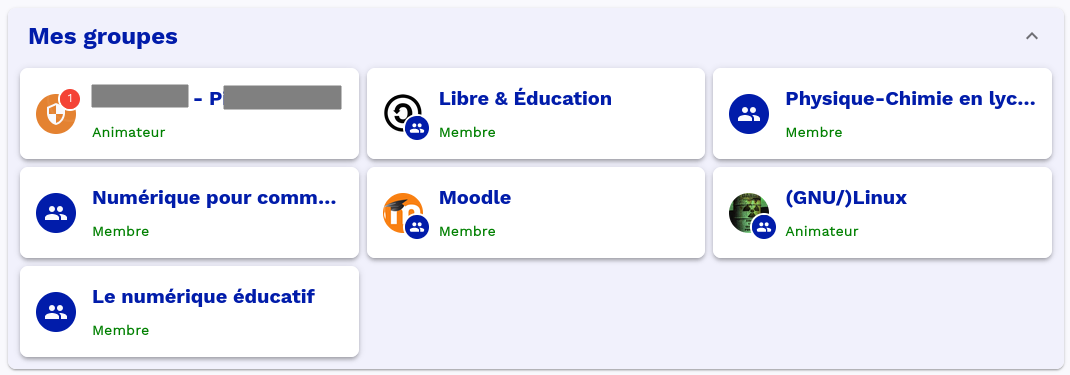
\includegraphics{./Captures/portail.accueil.mes.groupes.png}
	\caption{Les groupes ajoutés à mon profil.}
\end{figure}

Vous aurez noté sur le groupe du haut, à gauche, la présence d'un 1 dans un cercle rouge. 
Dans ce groupe modéré puisque de couleur orange où je suis animateur --comprendre administrateur-- il y a une notification. 
En l'occurrence il s'agit ...

\paragraph{Notez la présence d'un \^{} en haut à droite.}
Celui-ci permet de replier la zone consacrée à l'affichage de mes groupes.

\subsection{Gérer mes groupes}
La gestion des groupes s'effectue à partir du menu du profil. 
Bien évidemment, il s'agit de gérer les groupes dont on est administrateur ou modérateur, pas simple utilisateur
\begin{figure}
	\centering
	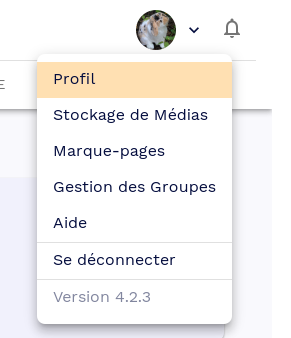
\includegraphics[width=0.3333\linewidth]{./Captures/menu.profil.png}
%	\caption{}
\end{figure}

\subsection{Détails d'un groupe}
En cliquant sur un des groupes, au hasard un de ceux administrés, voici les détails qui s'affichent. 
Ce tableau de bord complet montre tous les réglages et les options auxquelles il est possible d'accéder.
\begin{figure}
	\centering
	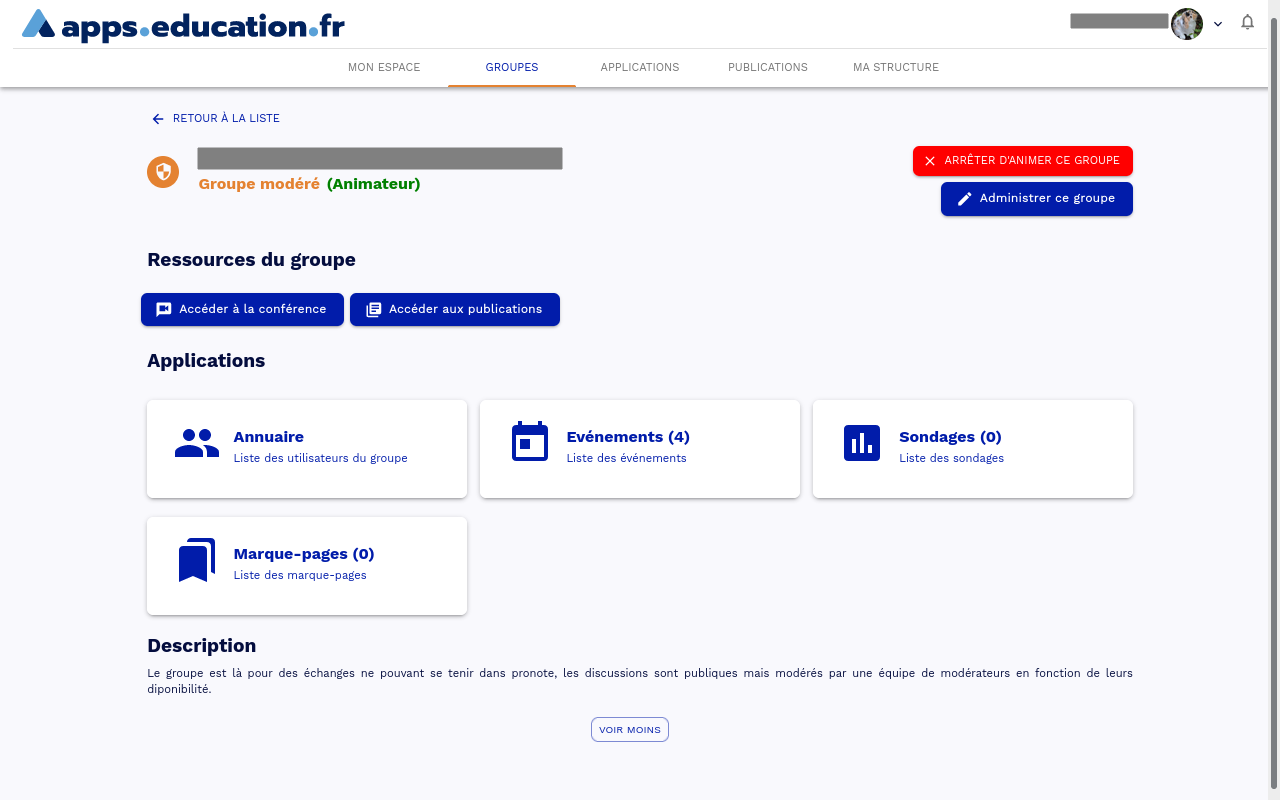
\includegraphics{./Captures/portail.groupe.affichage.details.png}
	\caption{L'intégralité des détails d'un groupe.}
\end{figure}


%%portail-ajout-application.tex
\section{Ajouter une application au profil}
Cette fois-ci c'est l'onglet \bsc{application} qui devra être sélectionnée.
\begin{figure}
	\centering
	
\includegraphics[width=\linewidth]{./Captures/portail.barre.seule.png}
%	\caption{}
\end{figure}
Dès lors, la liste des applications disponible apparaît avec des icônes permettant de filtrer par centre d'intérêt.
\begin{figure}
	\centering
	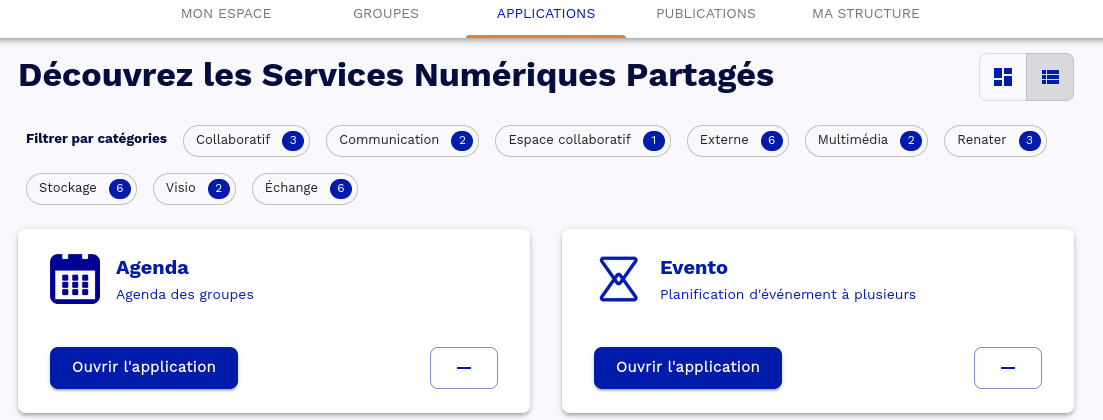
\includegraphics{./Captures/portail.applications.selection.png}
	\caption{sélectionner des applications}
\end{figure}
La capture précédente montre que les deux applications, \textbf{Agenda} et \textbf{Evento} sont déjà ajoutées à mon profil car sinon l'icône en bas à droite serait un ``+'' pour l'ajouter, alors que là c'est un ``--'' qui est visible me permettant de retirer l'application du profil.
\begin{figure}
 	\centering
 	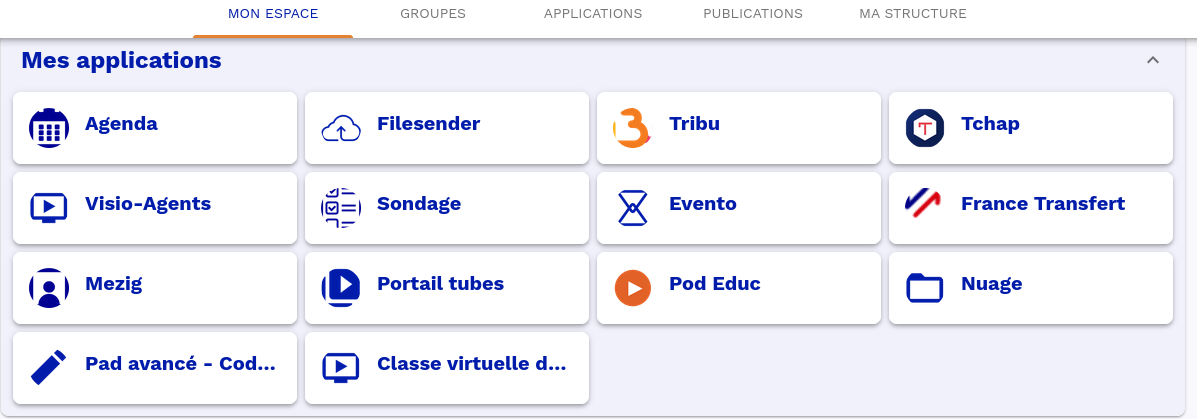
\includegraphics{./Captures/portail.mes.applications.png}
 	\caption{Les applications visibles et accessibles dans mon profil.}
 \end{figure}
Il est évidemment possible de retirer toute application du profil lorsque l'envie vous prendra.

% portail-ajout-bookmarks.tex
\section{Ajouter des liens extérieurs}
Parfois certaines applications en ligne ne sont pas pensées pour être intégrée au sein du projet Apps. 
Dans mon cas, le lien vers notre outil de gestion des notes, bulletins, cahiers de textes et absences, ou encore un environnement de développement de documents en \LaTeX{} n'est pas non plus disponible, mais, grâce à l'outil d'ajout de bookmarks, il est possible de les intégrer au sein du portail.

Comme pour la gestion des groupes, tout va commencer sur le menu du profil en haut à droite.
\begin{figure}
	\centering
	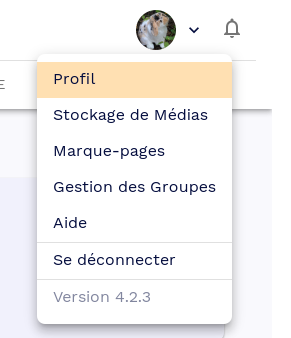
\includegraphics[width=0.3333\linewidth]{./Captures/menu.profil.png}
%	\caption{}
\end{figure}
et cette fois-ci c'est le choix ``Marque-pages'' qui va être choisi. 

\subsection{Descriptif de la fenêtre}
Une fois la ligne cliquée, une zone ressemblant à cet espace, mais vide bien sûr au début, va s'afficher. 
En voici un descriptif rapide.
\begin{figure}
	\centering
	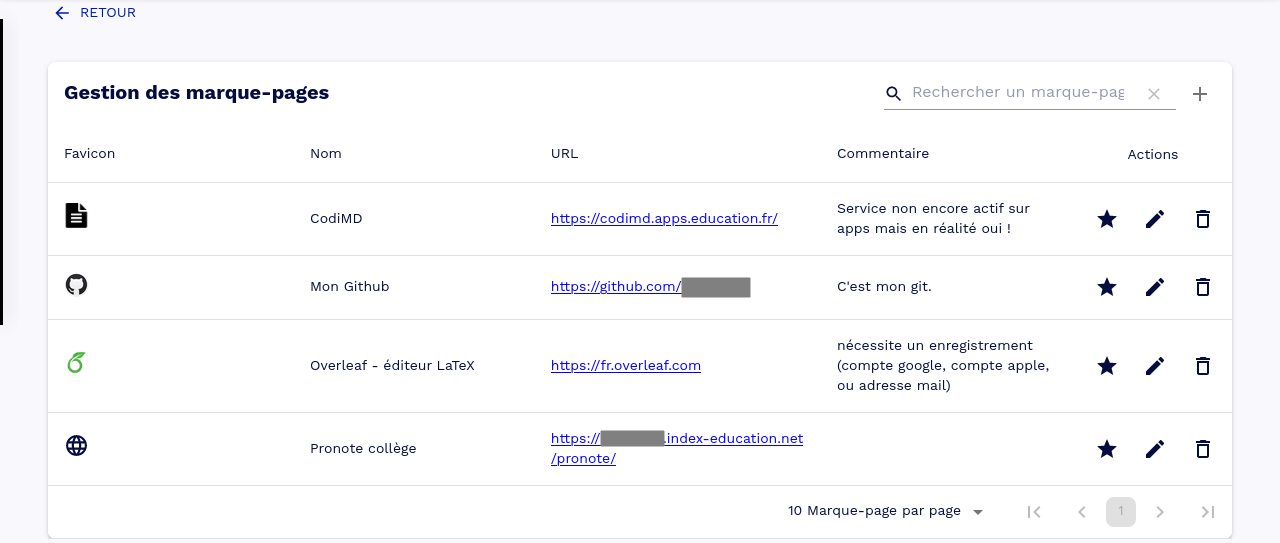
\includegraphics{./Captures/portail.marque.pages.gestion.png}
	\caption{Les marque-pages actuellement saisis dans mon profil}
\end{figure}
\begin{itemize}
	\item Situé en haut à gauche un lien de Retour permet de revenir à l'accueil,
	\item En haut vers la droite, un champ de recherche avec une loupe à sa droite permet de retrouver un lien si vous avez de nombreux liens déjà enregistrés,
	\item tout à droite, un + permet la création d'un nouveau marque page,
	\item la zone centrale affiche, ligne à ligne chaque marque page, les détails sont expliqués là $\rightarrow$ \ref{subsec-detail-bookmark},
	\item en bas à droite une ligne de navigation permet d'aller de page en page ou d'en sélectionner une lorsque beaucoup de liens auront été ajoutés et qu'ils ne tiendront plus sur une ligne unique.
\end{itemize}

\subsection{Détails d'un marque page} \label{subsec-detail-bookmark}
Voici l'examen détaillé d'une ligne de marque-pages, l'exemple du lien vers le site \emph{overleaf}.
\begin{figure}
	\centering
	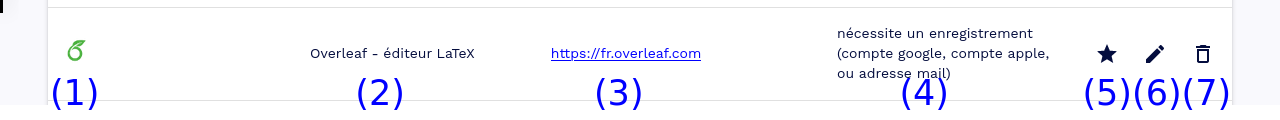
\includegraphics{./Captures/portail.marque.pages.exemple.png}
	\caption{Un exemple de marque-page, vers le site Overleaf}
\end{figure}
La ligne comporte sept zones différentes, voici leur explication de gauche à droite.
\begin{enumerate}
	\item icône du site web en question, sinon un icône générique,
	\item nom donné par moi-même au marque page,
	\item adresse internet du site,
	\item descriptif saisi par moi-même lors de la création du marque page,
	\item marque cet élément comme devant être parmi les favoris donc présent dans la page d'accueil, si l'étoile est creuse, le marque page reste ici, si elle est pleine, alors non seulement il sera présent dans la liste mais aussi apparaîtra en bas de l'onglet d'accueil,
	\item le stylo permet de modifier ultérieurement les détails du marque-page saisis lors de sa création,
	\item comme on peut aisément le deviner, l'icône poubelle permet d'effacer le marque-page, la capture suivante montre d'ailleurs le résultat.
\end{enumerate}
\begin{figure}
	\centering
	
\includegraphics{./Captures/portail.marque.pages.suppression.png}
	\caption{Suppression d'un marque page en attente de ma validation}
\end{figure}
L'appui sur $\surd$ validera l'action de suppression, sur $\times$ vous aurez simplement le retour à la liste des marque pages sans suppression.

De retour à l'écran d'accueil, vous aurez, en bas du profil, tous les marque-pages marqués comme favoris apparaissent.
\begin{figure}
	\centering
	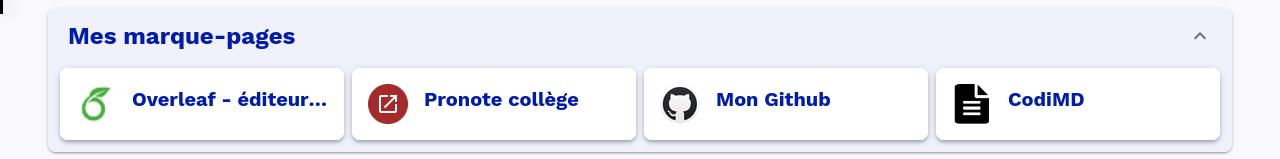
\includegraphics{./Captures/portail.accueil.mes.favoris.png}
	\caption{Mes marque-pages favoris affichés dans le profil.}
\end{figure}

\subsection{Création d'un marque-pages}
En cliquant sur le ``+'' à droite de la zone de recherche, elle-même en haut à droite de la fenêtre, cette mini fenêtre va s'afficher centralement.
\begin{figure}
	\centering
	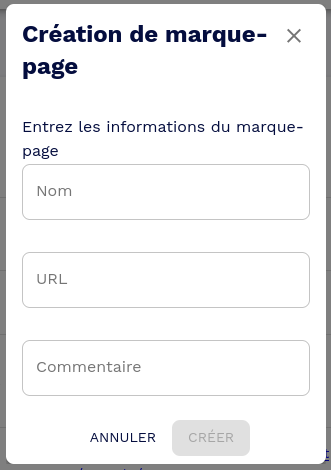
\includegraphics[width=0.333\linewidth]{./Captures/portail.marque.pages.creation.png}
	\caption{Création d'un marque page, pour l'instant vide.}
\end{figure}
Les seules indications importantes consistent à bien remplir tous les champs d'une part et surtout de bien ajouter \texttt{https://} ou \texttt{http://} en début d'adresse, le plus simple étant de copier-coller l'adresse affichée dans la barre éponyme du navigateur internet.

% portail-ajout-media.tex
\section{Ajouter des médias au profil}
En passant par la ligne de \textbf{stockage des média}, vous accéderez à une page spécifique montrant toutes les images que vous souhaitez stocker dans votre profil, hors du nuage étudié dans le chapitre idoine. 
Notez deux limitations :
\begin{itemize}
	\item l'espace maximum alloué est 100~Mo,
	\item chaque item ne peut pas dépasser la taille limite de 3~Mo
\end{itemize}
\begin{figure}
	\centering
	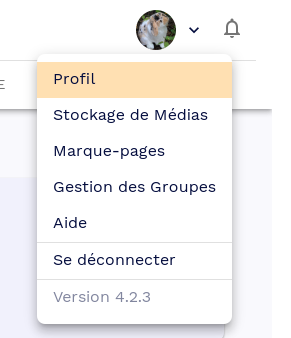
\includegraphics[width=0.3333\linewidth]{./Captures/menu.profil.png}
%	\caption{}
\end{figure}

\subsection{Ajouter un média}
Il existe deux méthodes pour ajouter un media à cet espace, le plus facile est d'ouvrir une fenêtre de l'explorateur de fichiers devant le navigateur, d'y sélectionner un ou plusieurs éléments, puis de les faire glisser sur la fenêtre du navigateur, les fichiers seront alors ajoutés à la liste des éléments présents.

L'autre méthode consiste à appuyer sur l'icône + à droite de la fenêtre, vers le haut.
\begin{figure}
	\centering
	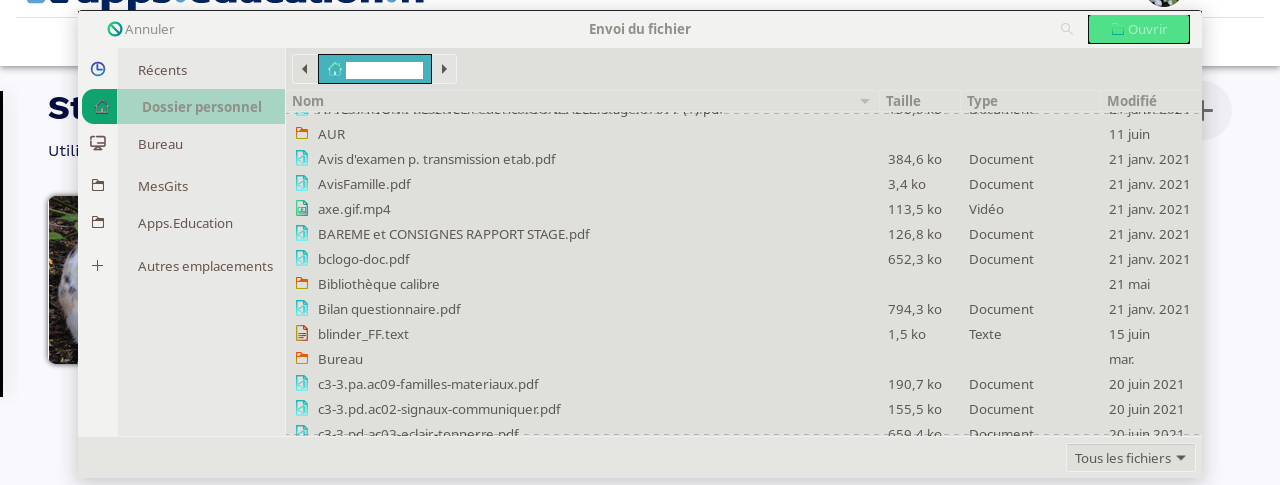
\includegraphics{./Captures/portail.stockage.medias.explorateur.png}
	\caption{L'appui sur ``+'' ouvre le navigateur local, ici en négatif car thème sombre originalement.}
\end{figure}
Une fenêtre de l'explorateur s'ouvrira, invitant l'utilisateur à choisir des éléments pour les y monter, comme le montre la capture plus haut
\begin{figure}
	\centering
	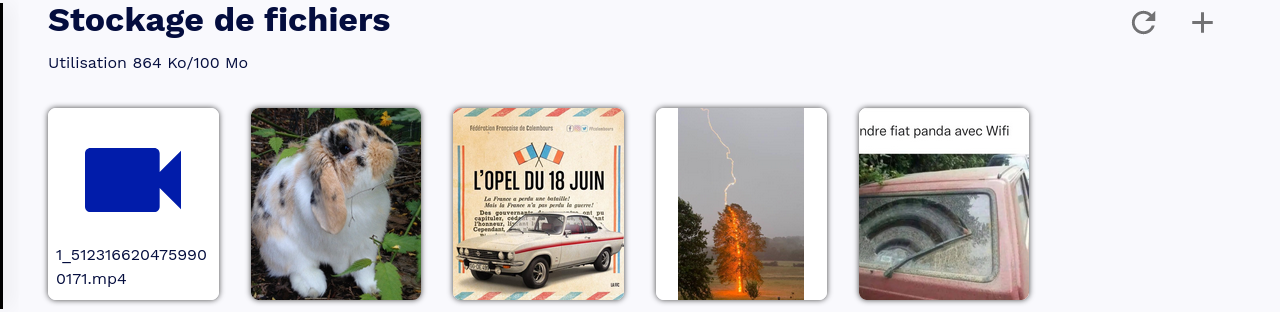
\includegraphics{./Captures/portail.stockage.medias.exemples.png}
	\caption{Affichage de quelques exemples déjà stockés sur mon profil.}
\end{figure}

\subsection{Gérer un média}
En sélectionnant un média, une mini-fenêtre de visualisation partielle (pour les images) ou de lecture (pour les vidéos) apparaît, elle se présente comme l'exemple qui suit.
\begin{figure}
	\centering
	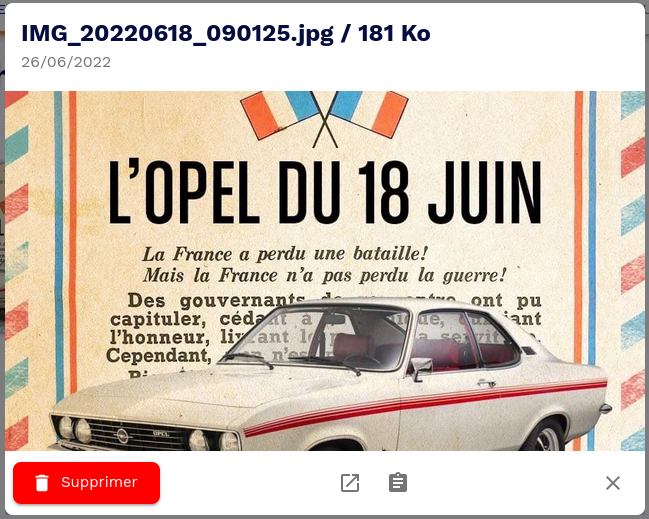
\includegraphics[width=0.500\linewidth]{./Captures/portail.stockage.medias.exemple.seul.png}
	\caption{Affichage d'un exemple de média stocké.}
\end{figure}
Vous aurez noté en haut le nom et la taille du document, quant à la partie basse elle présente une barre de gestion.
\begin{figure}
	\centering
	
\includegraphics[width=0.500\linewidth]{./Captures/portail.stockage.medias.barre.gestion.png}
	\caption{Les options de gestion d'une image stockée.}
\end{figure}
La barre de gestion des média affiche 4 options, de gauche à droite~:
\begin{itemize}
	\item un gros bouton rouge pour supprimer le média,
	\item un icône permettant d'afficher --sur mon navigateur cela déclenche le téléchargement-- du média dan sa totalité,
	\item un icône permettant de copier l'adresse de ce média,
	\item une croix pour fermer cette fenêtre.
\end{itemize}

\paragraph{Suppression d'un media.}
La suppression d'un média n'est pas directe et nécessite une double confirmation, en appuyant sur le gros bouton rouge, un compte à rebours de trois seconde s'enclenche pour valider cette suppression. 
À la fin du délais, si un second clic n'est pas venu attester le choix, la suppression n'est pas effective.
\begin{figure}
	\centering
	
\includegraphics[width=0.500\linewidth]{./Captures/portail.stockage.medias.suppression.png}
	\caption{Suppression d'un média, êtes-vous sûr(e) ?}
\end{figure}


% portail-publications.tex
\section{Mes publications.}
Dans l'onglet \bsc{publications} sont regroupées toutes les publications que vous avez rédigées, publications forcément associées à un groupe.
\begin{figure}
	\centering
	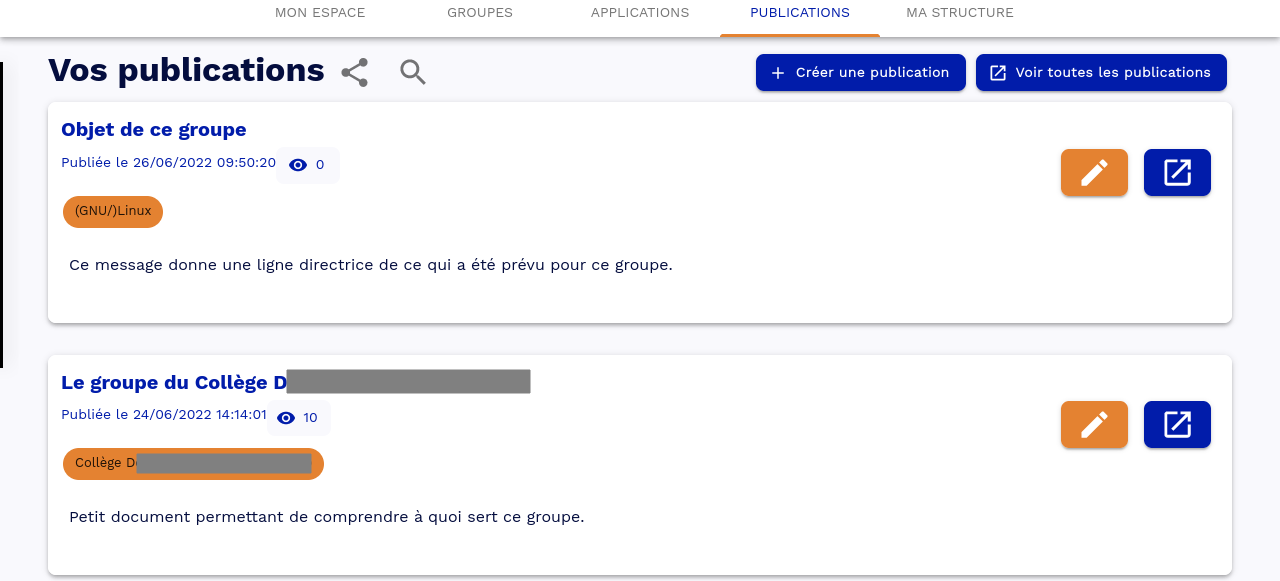
\includegraphics{./Captures/portail.publications.exemples.png}
	\caption{Exemples de publications personnelles.}
\end{figure}
Les seules options importantes sont regroupées vers la droite, il s'agit des gros boutons bleus pour
\begin{itemize}
	\item[+] Créer une publication
	\item[$\square$] Voir toutes les publications
\end{itemize}

Au sein d'une ligne de publication, les deux icônes importantes sont l'icône orange pour modifier une publication déjà rédigée, et pour afficher cette publication

\subsection{Créer une publication}
Lors de l'appui sur le bouton de création, une nouvelle fenêtre s'ouvre et les différents champs apparaissent. 
\begin{figure}
	\centering
	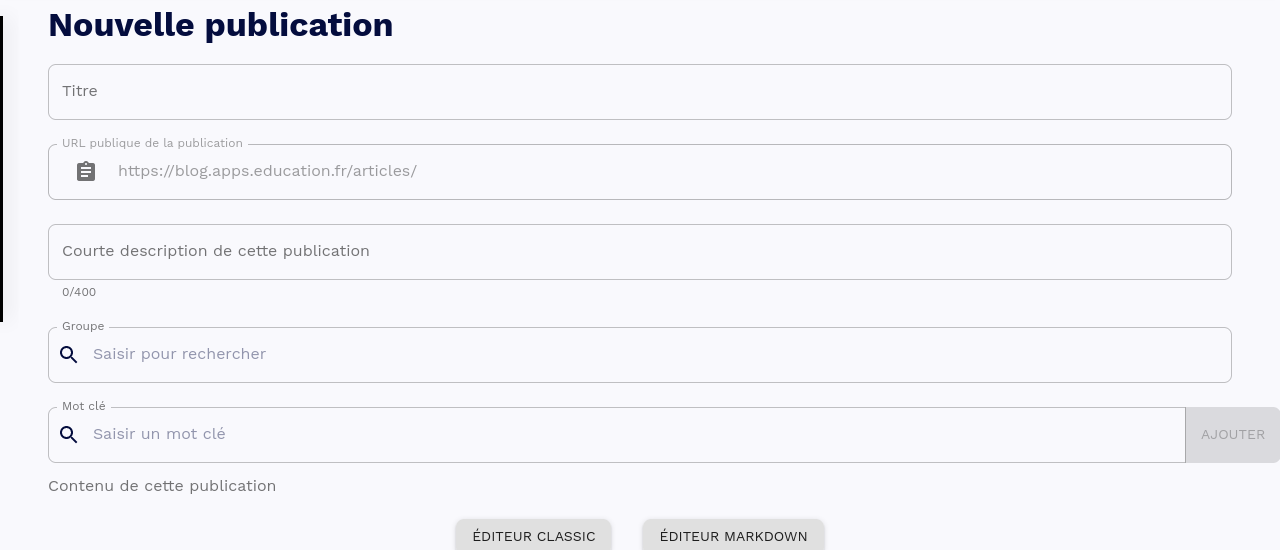
\includegraphics{./Captures/portail.publications.creer.publication.1.png}
	\caption{La première partie lors de la création d'une publication.}
\end{figure}
Parmi eux certains sont forcément obligatoires, en l'occurrence le titre bien sûr mais également le groupe dans lequel cette publication apparaîtra.

La partie inférieure de la fenêtre affiche deux options pour la publication et des boutons correspondants, à savoir l'éditeur classique ou l'éditeur markdown.

\paragraph{L'éditeur classique} affiche une barre d'options de formatage et d'inclusion d'objets classiques comme des listes numérotées ou pucées, des  permet aussi l'insertion d'en-têtes dans la publication (titre, sous-titre,  ...)
\begin{figure}
	\centering
	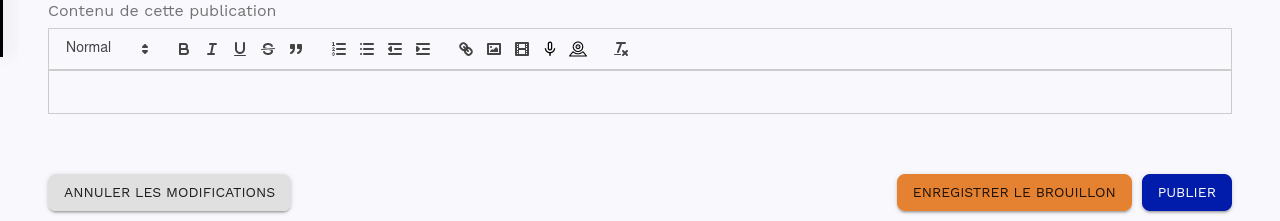
\includegraphics{./Captures/portail.publications.creer.publication.2.classique.png}
	\caption{La seconde partie de la création d'une publication : l'éditeur classique}
\end{figure}
De gauche à droite les icônes permettent :
\begin{itemize}
	\item de structurer le texte sélectionné avec un niveau hiérarchique dans le document,
	\item de mettre la sélection en (on peut cocher plusieurs choix)
		\begin{itemize}
		\item gras
		\item italique
		\item souligné
		\item barré
		\end{itemize}
	\item d'ajouter une citation
	\item d'ajouter une liste numérotée
	\item d'ajouter une liste pucée
	\item de diminuer le retrait du texte sélectionné
	\item d'augmenter le retrait du texte sélectionné
	\item d'ajouter un lien vers une ressource sur internet,
	\item d'insérer une image
	\item d'insérer une vidéo
	\item d'insérer un fichier audio
	\item d'enregistrer et insérer une vidéo (si la webcam existe sur l'ordinateur)
	\item de supprimer les mises en forme de la sélection
\end{itemize}

\paragraph{L'éditeur Markdown}
Markdown est un langage de balisage léger permettant de l'insertion d'objets et du formatage. 
Le chapitre \ref{chap-codimd} se réfère à ce langage tellement pratique qu'il est devenu mon outil de prise de notes pendant les réunions.
\begin{figure}
	\centering
	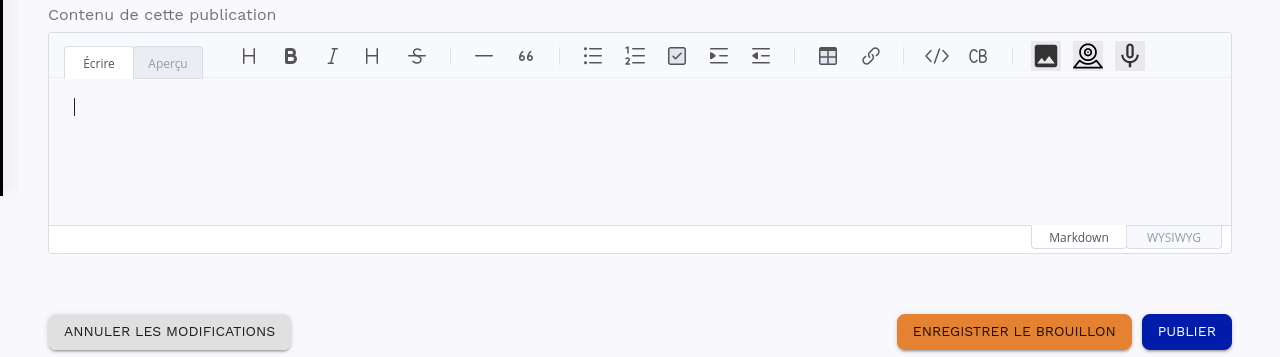
\includegraphics{./Captures/portail.publications.creer.publication.2.markdown.png}
	\caption{}
\end{figure}

\paragraph{Les deux modes acceptés en Markdown.} 
Ce sont le mode Markdown et le mode WYSIWYG\footnote{%
WYSIWYG : \emph{What You See Is What You Get} est un acronyme désignant une famille d'outils numériques, généralement des traitements de textes, où vous avez le formatage et le rendu en même temps que vous le saisissez. 
Cette famille diffère d'autres langages ou logiciels de traitement de texte comme Markdown, Restructured Text ou encore \TeX{} et \LaTeX{} (entre autres) où le formatage est signifié par des balises mais le rendu n'est visible qu'après compilation du document.
}.

L'éditeur Markdown offre la barre suivante avec de gauche à droite~:
\begin{figure}
	\centering
	
\includegraphics{./Captures/portail.publications.creer.publication.barre.markdown.png}
	\caption{L'éditeur Markdown}
\end{figure}
\begin{itemize}
	\item gestion des en-têtes (titre, sous-titre, ...), 
	\item gras,
	\item italique,
	\item choix de la couleur du texte,
	\item texte barré,
	\item ligne horizontale,
	\item citation,
	\item liste pucée,
	\item liste numérotée,
	\item case de tâche à cocher,
	\item augmentation du retrait du texte,
	\item diminution du retrait du texte,
	\item insertion d'un tableau,
	\item insertion d'un lien vers l'extérieur,
	\item insertion d'un code en ligne,
	\item insertion d'un code en bloc,
	\item ajout d'un media (comprendre image),
	\item enregistrement et ajout d'une vidéo,
	\item enregistrement et ajout d'une séquence audio
\end{itemize}

L'éditeur WYSIWYG offre la barre suivante, certaines options de l'éditeur markdown sont soit absentes, soit inactives (grisées clairement)
\begin{figure}
	\centering
	
\includegraphics{./Captures/portail.publications.creer.publication.barre.wysiwyg.png}
	\caption{L'éditeur Markdown-Wysiwyg}
\end{figure}

\paragraph{Enregistrement}
Une fois la note saisie entièrement le bas de la fenêtre offre trois choix, celui de l'annulation, celui de l'enregistrement en tant que brouillon ou bien celui de la publication, comme le montre la capture suivante.
\begin{figure}
	\centering
	
\includegraphics{./Captures/portail.publications.creer.publication.3.png}
	\caption{\emph{this is your last chance}}
\end{figure}

\subsection{Voir toutes les publications}
L'autre bouton important de l'onglet publications ouvre une nouvelle fenêtre, ou un nouvel onglet suivant la configuration de votre navigateur, pour afficher les derniers articles du blog.
\begin{figure}
	\centering
	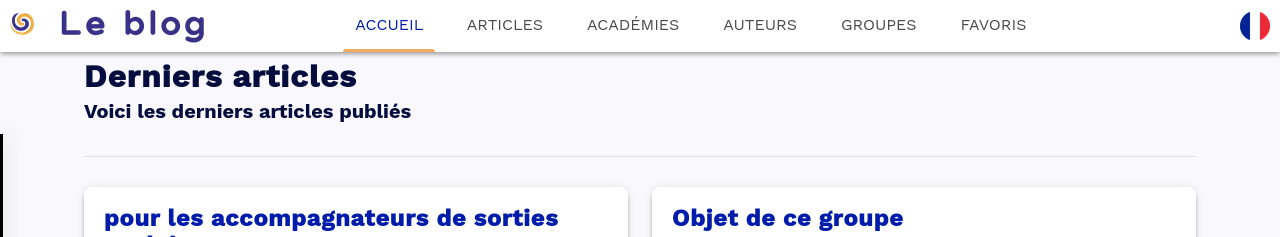
\includegraphics{./Captures/portail.publications.afficher.toutes.le.blog.png}
	\caption{Les derniers articles du blog}
\end{figure}

Notez que la barre du haut de la fenêtre est également changée, puisque cette fois-ci c'est celle qui suit qui s'affiche.
\begin{figure}
	\centering
	
\includegraphics{./Captures/portail.publications.afficher.toutes.le.blog.barre.png}
	\caption{La barre du blog}
\end{figure}
Elle permet d'afficher de gauche à droite, l'accueil avec les dernières publications, l'intégralité des publications avec un outil de filtrage par tags, les régions académiques avec les publications rattachées par région ou structure (comme CANOPÉ par exemple), la liste des auteurs et le nombre d'article qu'ils ont publié, la liste des groupes et le nombre de publications associées au groupe, et pour finir les publications lues et marquées comme favorites par vos soins.

% portail-structure.tex
\section{Ma structure}
Chaque structure régionale peut proposer des outils qui lui sont propres et intégrés au portail, cela se retrouvera dans l'onglet \bsc{ma structure}, ici la région nouvelle-aquitaine propose un outil de visioconférence, en cliquant sur le plus en bas à droite de la vignette (le plus devenant alors un moins) l'outil est ajouté au profil.
\begin{figure}
	\centering
	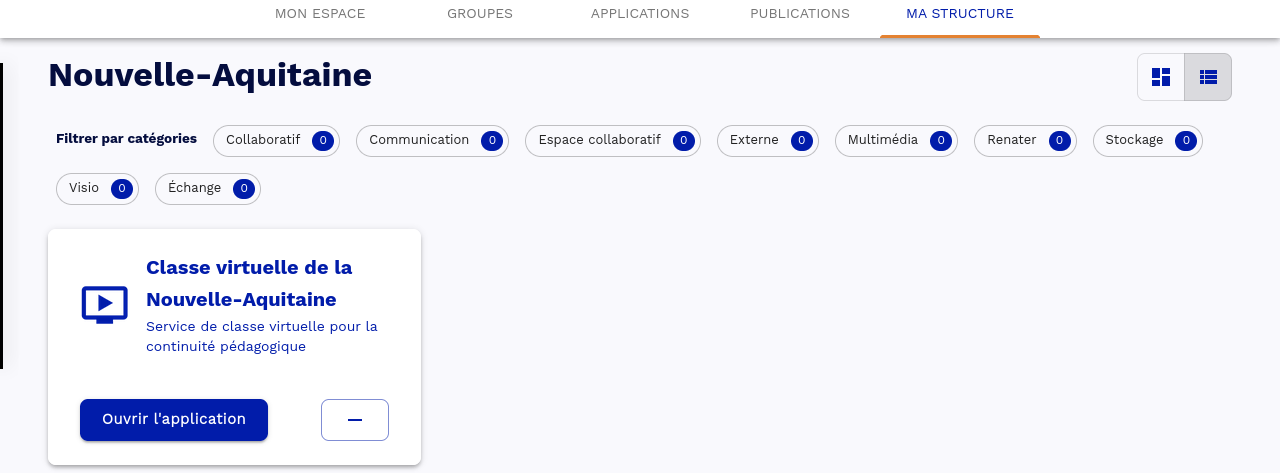
\includegraphics{./Captures/portail.accueil.ma.structure.png}
	\caption{Les applications et autres offres de la part de ma structure de rattachement.}
\end{figure}


Enfin, lorsque vous désirez quitter votre profil, surtout si vous êtes sur un ordinateur public, en passant par la dernière ligne du menu contextuel du profil, vous accéderez à la ligne de déconnexion. 
Celle-ci est primordiale pour une bonne hygiène informatique et quelques règles élémentaires de sécurité numérique.
\begin{figure}
	\centering
	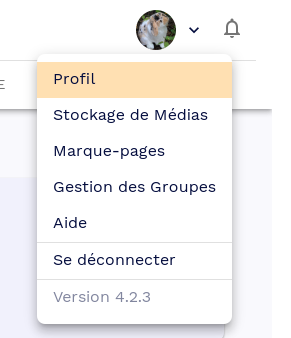
\includegraphics[width=0.3333\linewidth]{./Captures/menu.profil.png}
%	\caption{}
\end{figure}